%!TeX root=../tese.tex
%("dica" para o editor de texto: este arquivo é parte de um documento maior)
% para saber mais: https://tex.stackexchange.com/q/78101

\chapter{Automated Refactoring}
\label{chap:related_work}




The ``code processing community''\footnote{There does not seem to be a consensus for a name for the area, some common names are big code and programming language processing.} may be comparatively small to the NLP community, but it is not by any means non-existent. This chapter will present related work to our goal of automating function extractions, our objective is to situate the reader about recent relevant developments and to explicitate how this project differs from recent and current works in the area.



\section{Rename Method}
The rename method refactoring is one of the most commonly performed refactorings \citep{mauricio_paper}, an illustration of it can be seen in Fig.~\ref{fig:rename_method}. Due to it essentially being an act of naming something for humans to read, it is a task that can be greatly benefited from natural language processing techniques and insights. 


\begin{figure}[!ht]
\centerline{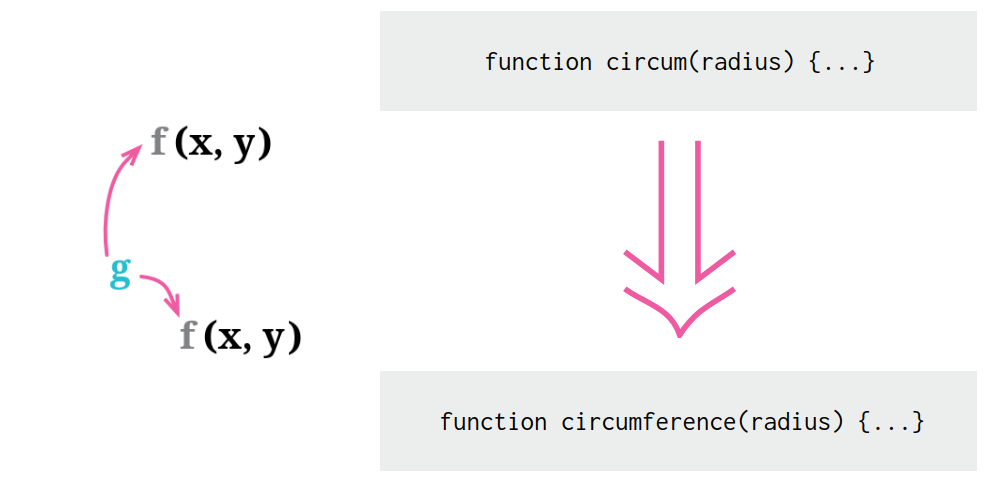
\includegraphics[width=0.6\textwidth]{figuras/rename_method.png}}
\caption{Illustration of a refactoring of the \textit{Rename Method} type. Illustration adapted from \citet{rename_method}.}
\label{fig:rename_method}
\end{figure}


In this section we will explore a few recent works that attained state of the art performance in this task at the time of their publication. But since many of them utilize an AST to achieve that, we will start by explaining what an AST is.



\subsection{AST}

For source code to become an executable program it needs to be translated into a low level language capable of being run by the machine or into machine code directly. A common approach is to write a compiler that will take the source code and compile it into an executable binary that may be used any time. A compiler is composed of numerous processing steps that can be somewhat separated into 2 categories: analysis and synthesis \citet{batata}.
The analysis part pre-processes the inputted code and generates an intermediary representation of it to be used by the synthesis step. If during the analysis the code is found to be grammatically incorrect (in respect to the programming language formal grammar) or to have any other problem of lexical, syntactical or semantic nature it will abort the compilation process and report to the user an error message. By the end of a successful analysis step an intermediary representation of the source code will be generated, e. g. an Abstract Syntax Tree.


The AST is created by taking its concrete counterpart the concrete parse tree, also known as a parse tree, and removing any redundant or unnecessary information such as idiosyncrasies related to the source language or precedence and punctuation tokens (such as parenthesis in arithmetic expressions or ``;'' to denote the end of a statement) that are made unnecessary once the parse tree is built. 
Or as it is succinctly described in the book \textit{Modern Compiler Implementation in Java}:


\begin{myquote}
\textit{The abstract syntax tree conveys the phrase structure of the source program, with all parsing issues resolved but without any semantic interpretation.} \\\citet{java_tigre}
\end{myquote}


It is no surprise that ASTs are often selected as a starting point for code embeddings, as it captures the structure of the source code that is not readily available when analyzing solely the source code.
An AST can be seen in Fig.~\ref{fig:ast} and its corresponding source code in Listing~\ref{listing:hello}.




\begin{listing}[!ht]
\inputminted[linenos, breaklines]{java}{conteudo/code/hello.java}
\caption{Small Java script, its AST can be seen in Fig.~\ref{fig:ast}.}
\label{listing:hello}
\end{listing}



\begin{landscape}
\begin{figure}[!ht]
\centerline{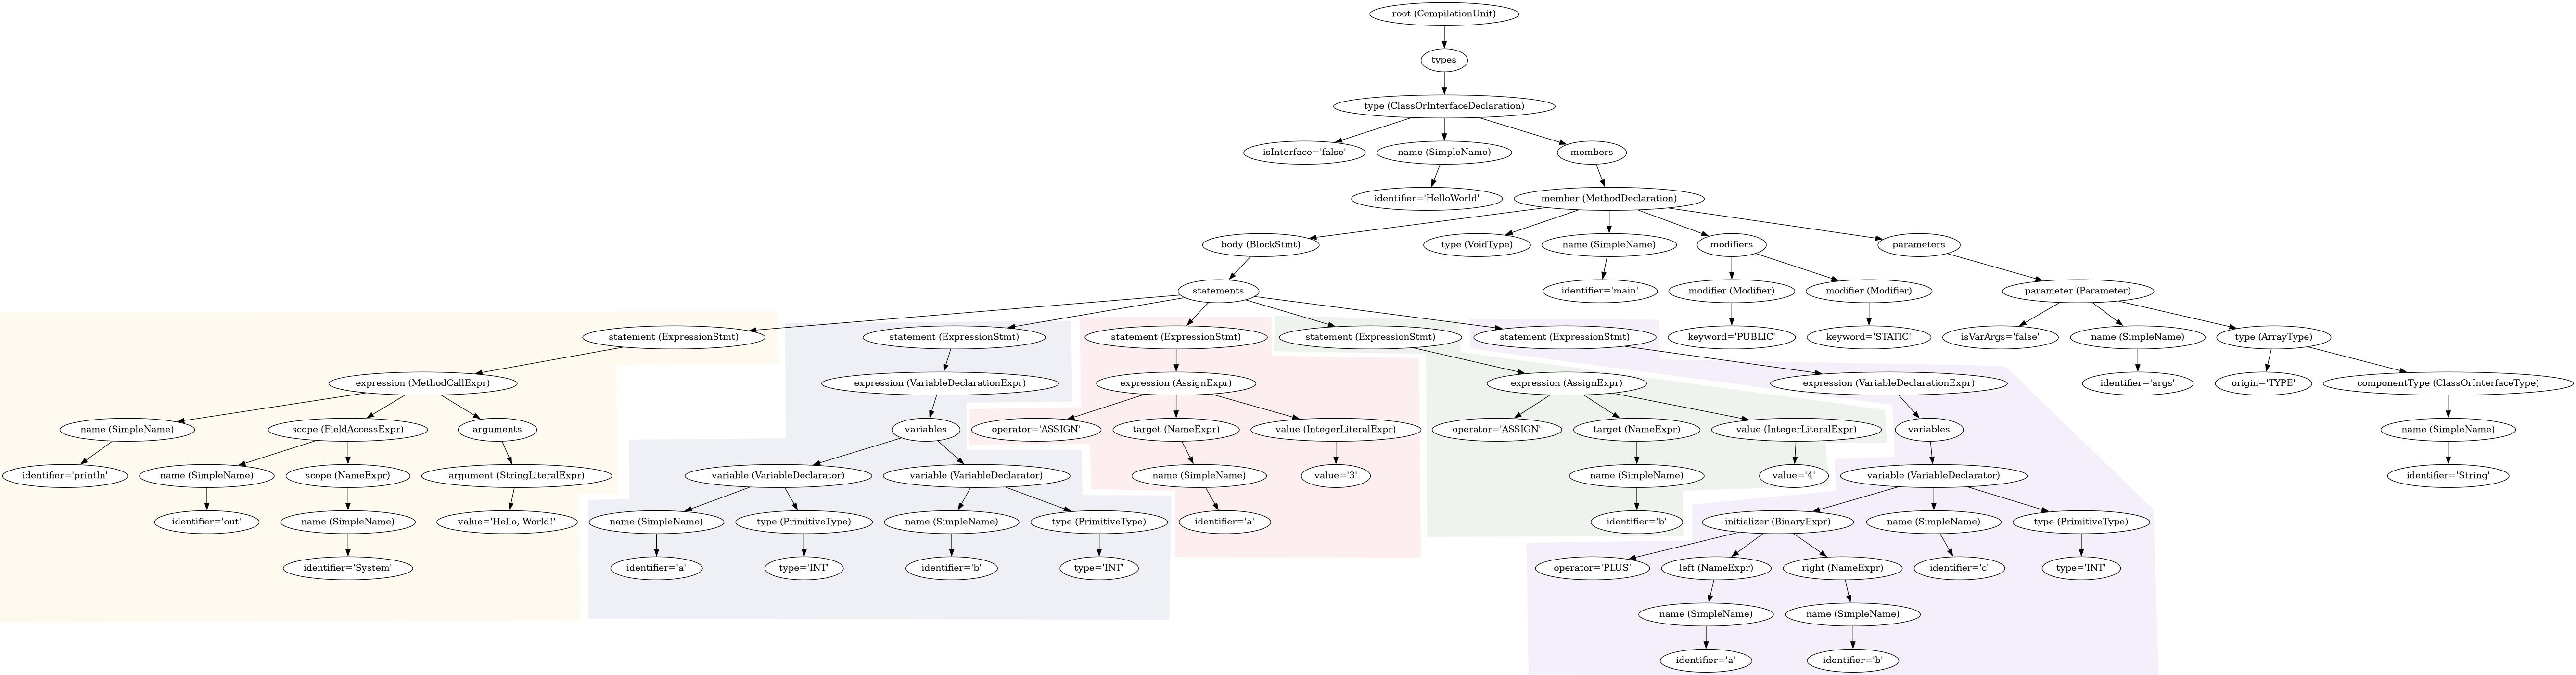
\includegraphics[height=0.5\textheight]{figuras/hello_astfinal_colorido.png}}
\caption{AST of Listing~\ref{listing:hello}. In an attempt to make the AST more intuitive and easier to read for those that never worked with them, we colored the sub-trees that correspond to the lines of the function body with one color per corresponding line\footnote{Since Java utilizes ``;'' to denote the end of a statement, multiple statements could be present in a single line of code but the AST would break down each line in its composing statements with one sub-tree for each. The existence of different lines is simply syntactic sugar, all Java programs could be expressed in single lines}. AST printed through the \texttt{dot} utility and the \texttt{JavaParser}  package, the code utilized to print the AST is available at Appendix~\ref{an:astcoisas} as Listing~\ref{listing:printer}.}
\label{fig:ast}
\end{figure}
\end{landscape}




\subsection{code2vec and code2seq}

Code2vec \citep{code2vec} is an algorithm that generates code embeddings, i.e. distributed representation of code and similar in spirit to word2vec. 
A path-based attention model was developed for learning embeddings of arbitrary-sized snippets of code, which was done through the use of paths in the program’s abstract syntax tree as a representation for code.
The authors managed to leverage the underlying structure of the programming language to develop a scalable and efficient code embedding generator.


\begin{figure}[!ht]
\centerline{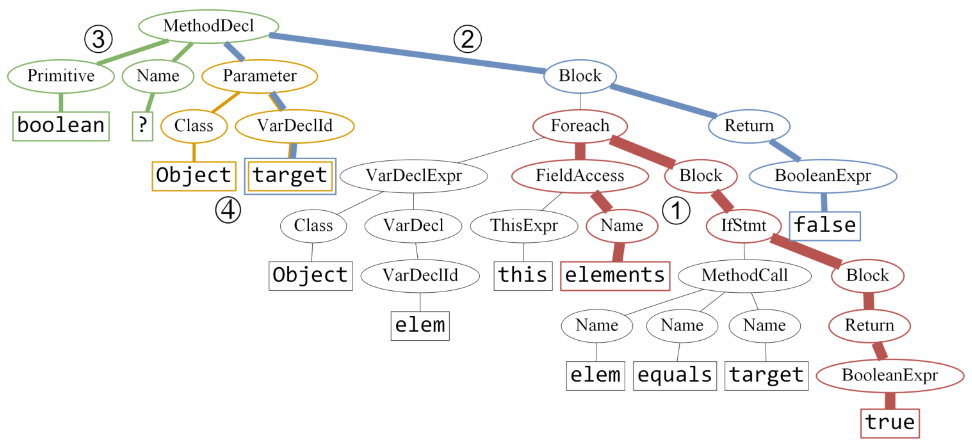
\includegraphics[width=\textwidth]{figuras/code2vecpaths.png}}
\caption{Illustration of the path-based attention model from code2vec. The width of each colored path is proportional to the attention it was given (red 1: 0.23, blue 2: 0.14, green 3: 0.09, orange 4: 0.07). \citep{code2vec}}
\label{fig:code2vec}
\end{figure}

Similarly to word2vec, this representation was successful in learning syntactic and semantic information, being able to generate analogies such as ``$receive$ is to $send$ as $download$ is to: $upload$''. 

Furthermore, code2vec was shown to be capable of capturing the resulting effect of two different function calls in succession, e.g. when given the embedding for the functions ``equals'' and ``toLower'', their sum is predicted to be equivalent to the function ``equalsIgnoreCase'', i.e. ``$equals$ + $toLower \approx  equalsIgnoreCase$''. %It is important to note that since the code2vec embeddings are generated from the program AST the function names are never used in the training process and as such the only information utilized is the underlying structural information captured by the AST and the path-based attention.


Code2seq \citep{code2seq} is another model created by the same group that built code2vec, building upon their previous findings and successes working with AST paths. It represents a code snippet as the set of compositional paths in its abstract syntax tree and uses attention to select the relevant paths while decoding.
This new approach achieved better performance than code2vec, achieving a new state of the art while expanding the abilities of their model. It is capable of performing code summarization, caption and documentation. 







\subsection{Code Transformer}

The code transformer model from \citet{code_transformer} has a more holistic approach, instead of utilizing the pure source code or the AST it chooses to do both. By utilizing what they define as context (source code) and structure (AST) they were able to combine two facets of programs and obtain state-of-the-art performance on monolingual code summarization in five languages and propose the first multilingual code summarization model.
This multilingual model substantially outperformed its mono-lingual variants on all programming languages of the study. 

The authors also noted that multilingual training only from context did not lead to the same improvements, highlighting the benefits of combining structure and context.
An overview of the code transformer structure can be seen in Fig.~\ref{fig:codetransf}.

\begin{figure}[!ht]
\centerline{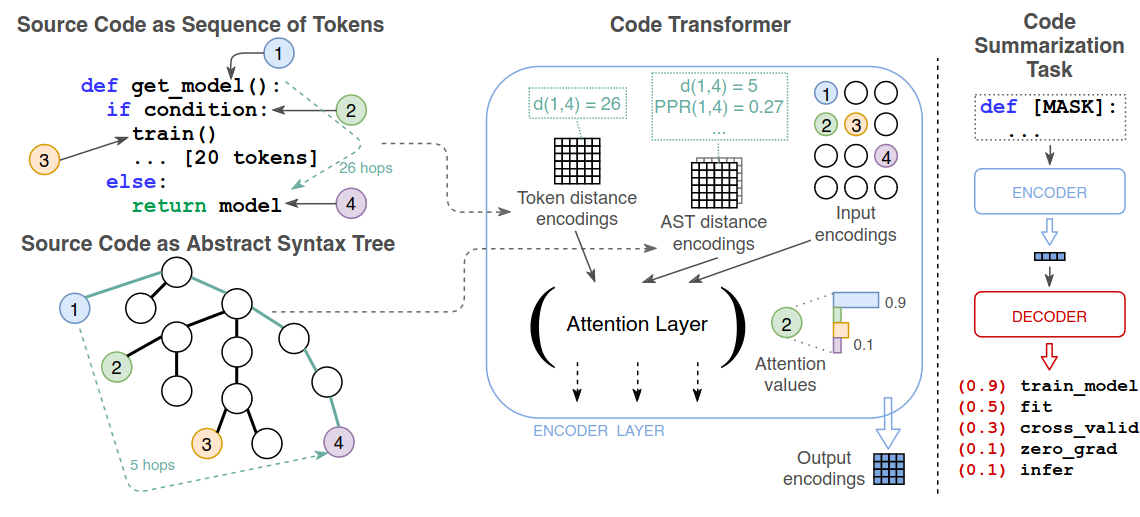
\includegraphics[width=\textwidth]{figuras/code-transformer.png}}
\caption{``\textbf{Left:} Sequence (Context) and AST (Structure) representation of an input code snippet. \textbf{Center:} The CODE TRANSFORMER jointly leverages the sequence of tokens and the Abstract Syntax Tree to learn expressive representations of source code. In addition to the input token and node embeddings the model uses different distances between the tokens, e.g., shortest paths on the AST or personalized PageRank, to reason about their relative positions. The output embeddings can be used for downstream tasks such as code summarization \textbf{(right)}.'' \citep{code_transformer}}
\label{fig:codetransf}
\end{figure}







\section{Github Copilot X, Code Whisperer and Code Assistants}

In recent years there has been an influx of code assisting tools based on machine learning models. Most of them are closed source with no details about their implementation, such as TabNine's autocompleter \citep{tabnine}, Amazon's CodeWhisperer code assistant \citep{whisperer} and Microsoft's Copilot, or even platform specific such as Replit's Ghostwriter \citep{ghost_writer}. With the release of Copilot X \citep{copilotx}, the latest iteration of the GitHub Copilot project, some details were made available to the public about its implementation but not that much is known besides the fact that they claim to use GPT-4.


Another interesting experimental project by the \citet{brushes} team are the code brushes , where the user can choose ``brushes'' to apply certain effects on code, such as making it more readable, adding types or including debugging statements, among other code transformations. Most of its brush operations are essentially refactorings, small operations with the intent of making code more readable and maintainable without altering its behavior. 
However, currently there is not a brush for function extractions.


These ``AI'' assisted tools have managed to achieve great popularity among developers, however due to their closed source nature, wait lists and paywalls, it is difficult to even try to compare them with the work developed in this project since we lack access to them and the knowledge about what is going on under the hood. The more flexible systems based on LLMs, such as Copilot X, could be tailored through prompts to attempt to realize function extractions, but doing so in a programmatical manner to measure its performance would be a challenge. We are still awaiting for the opportunity to test the Copilot X but even if we had access to it and achieved a good performance in the function extraction task there would be the doubt about the nature of this performance: is the model performing well or is it simply overfitted? Since our training, validation and test sets come from Java projects in GitHub, it would be hard to determine if the test files were never used during the Copilot X training leading to data snooping.

For these reasons, there won't be any comparisons between these tools and the models we developed, however we felt the need to mention them for the sake of completeness.





\section{Machine learning based code refactoring prediction}
\label{sec:mauricio}

Work from \citet{mauricio_paper} has shown that supervised machine learning methods are effective in predicting refactoring opportunities and, more importantly, such models can accurately model the refactoring recommendation problem. 
For this task, process and ownership metrics where shown to be essential for model creation, were the ownership metrics correspond to the suite proposed by \citet{ownership_metrics} and the process metrics are: quantity of commits, number of bug fixes, the sum of lines added, the sum of lines removed,  and number of previous refactoring operations.

Albeit an important milestone, it's important to emphasize that the model proposed on this work was only capable of predicting refactoring \textit{types} and \textit{opportunities}, not the refactoring operations themselves.
The models generated have also been shown to be robust with context change, i.e. a model trained in one context (e.g. Apache projects) can accurately predict refactoring opportunities on another context/project (e.g. F-droid projects). In Table~\ref{table:mau_modelos} we present the performance of the different models trained by \citet{mauricio_paper}.




\begin{table}[!ht]
\centering
\caption{The precision (Pr), recall (Re), and accuracy (Acc) of the different machine learning models, when trained and tested in the entire dataset (Apache + F-Droid + GitHub). Values range between [0,1]  \citep{mauricio_paper}. Table reconstructed from the original paper.}

\label{table:mau_modelos}

\resizebox{\textwidth}{!}{

\begin{tabular}{l c c c|c c c|c c c|c c c|c c c|c c c}
\hline & \multicolumn{3}{c}{$\begin{array}{c}\text { \textbf{Logistic} } \\
\text { \textbf{Regression} }\end{array}$} & \multicolumn{3}{c}{$\begin{array}{c}\text { \textbf{SVM} } \\
\text { \textbf{(linear)} }\end{array}$} & \multicolumn{3}{c}{$\begin{array}{c}\text { \textbf{Naive Bayes} } \\
\text {\textbf{ (gaussian)} }\end{array}$} & \multicolumn{3}{c}{$\begin{array}{c}\text { \textbf{Decision} } \\
\text { \textbf{Tree} }\end{array}$} & \multicolumn{3}{c}{$\begin{array}{c}\text { \textbf{Random} } \\
\text { \textbf{Forest} }\end{array}$} & \multicolumn{3}{c}{$\begin{array}{c}\text { \textbf{Neural} } \\
\text { \textbf{Network} }\end{array}$} \\
\hline & $\operatorname{Pr}$ & $\operatorname{Re}$ & $\operatorname{Acc}$ & $\operatorname{Pr}$ & $\operatorname{Re}$ & $\operatorname{Acc}$ & $\operatorname{Pr}$ & $\operatorname{Re}$ & $\operatorname{Acc}$ & $\operatorname{Pr}$ & $\operatorname{Re}$ & $\operatorname{Acc}$ & $\operatorname{Pr}$ & $\operatorname{Re}$ & $\operatorname{Acc}$ & $\operatorname{Pr}$ & $\operatorname{Re}$ & $\operatorname{Acc}$ \\
\hline \multicolumn{19}{l}{ \textbf{Class-level refactorings} } \\
Extract Class & 0.78 & 0.91 & 0.82 & 0.77 & 0.95 & 0.83 & 0.55 & 0.93 & 0.59 & 0.82 & 0.89 & 0.85 & 0.85 & 0.93 & 0.89 & 0.80 & 0.94 & 0.85 \\
 Extract Interface & 0.83 & 0.93 & 0.87 & 0.82 & 0.94 & 0.87 & 0.58 & 0.94 & 0.63 & 0.90 & 0.88 & 0.89 & 0.93 & 0.92 & 0.92 & 0.88 & 0.90 & 0.89 \\
 Extract Subclass & 0.85 & 0.94 & 0.89 & 0.84 & 0.95 & 0.88 & 0.59 & 0.95 & 0.64 & 0.88 & 0.92 & 0.90 & 0.92 & 0.94 & 0.93 & 0.84 & 0.97 & 0.89 \\
 Extract Superclass & 0.84 & 0.94 & 0.88 & 0.83 & 0.95 & 0.88 & 0.60 & 0.96 & 0.66 & 0.89 & 0.92 & 0.90 & 0.91 & 0.93 & 0.92 & 0.86 & 0.94 & 0.89 \\
 Move And Rename Class & 0.89 & 0.93 & 0.91 & 0.88 & 0.95 & 0.91 & 0.69 & 0.94 & 0.76 & 0.92 & 0.95 & 0.94 & 0.95 & 0.95 & 0.95 & 0.88 & 0.94 & 0.91 \\
 Move Class & 0.92 & 0.96 & 0.94 & 0.90 & 0.97 & 0.93 & 0.67 & 0.96 & 0.74 & 0.98 & 0.96 & 0.97 & 0.98 & 0.97 & 0.98 & 0.92 & 0.97 & 0.94 \\
 Rename Class & 0.87 & 0.94 & 0.90 & 0.86 & 0.96 & 0.90 & 0.63 & 0.96 & 0.69 & 0.94 & 0.91 & 0.93 & 0.95 & 0.94 & 0.94 & 0.88 & 0.94 & 0.91 \\
\hline \multicolumn{19}{l}{ \textbf{Method-level refactorings} } \\
 Extract And Move Method & 0.72 & 0.86 & 0.77 & 0.71 & 0.89 & 0.76 & 0.63 & 0.94 & 0.69 & 0.85 & 0.75 & 0.81 & 0.90 & 0.81 & 0.86 & 0.79 & 0.85 & 0.81 \\
 Extract Method & 0.80 & 0.87 & 0.82 & 0.77 & 0.88 & 0.80 & 0.65 & 0.95 & 0.70 & 0.81 & 0.86 & 0.82 & 0.80 & 0.92 & 0.84 & 0.84 & 0.84 & 0.84 \\
 Inline Method & 0.72 & 0.88 & 0.77 & 0.71 & 0.89 & 0.77 & 0.61 & 0.94 & 0.67 & 0.94 & 0.87 & 0.90 & 0.97 & 0.97 & 0.97 & 0.77 & 0.85 & 0.80 \\
 Move Method & 0.72 & 0.87 & 0.76 & 0.71 & 0.89 & 0.76 & 0.63 & 0.93 & 0.70 & 0.98 & 0.87 & 0.93 & 0.99 & 0.98 & 0.99 & 0.76 & 0.84 & 0.78 \\
 Pull Up Method & 0.78 & 0.90 & 0.82 & 0.77 & 0.91 & 0.82 & 0.68 & 0.95 & 0.75 & 0.96 & 0.88 & 0.92 & 0.99 & 0.94 & 0.96 & 0.82 & 0.87 & 0.84 \\
 Push Down Method & 0.75 & 0.89 & 0.80 & 0.75 & 0.90 & 0.80 & 0.66 & 0.94 & 0.73 & 0.97 & 0.76 & 0.87 & 0.97 & 0.83 & 0.90 & 0.81 & 0.92 & 0.85 \\
 Rename Method & 0.77 & 0.89 & 0.80 & 0.76 & 0.90 & 0.80 & 0.65 & 0.95 & 0.71 & 0.78 & 0.84 & 0.80 & 0.79 & 0.85 & 0.81 & 0.81 & 0.82 & 0.81 \\
\hline \multicolumn{19}{l}{\textbf{Variable-level refactorings} } \\
Extract Variable & 0.80 & 0.83 & 0.82 & 0.80 & 0.83 & 0.82 & 0.62 & 0.94 & 0.68 & 0.82 & 0.83 & 0.82 & 0.90 & 0.83 & 0.87 & 0.84 & 0.89 & 0.86 \\
Inline Variable & 0.76 & 0.86 & 0.79 & 0.75 & 0.87 & 0.79 & 0.60 & 0.94 & 0.66 & 0.91 & 0.85 & 0.88 & 0.94 & 0.96 & 0.95 & 0.81 & 0.82 & 0.82 \\
Parameterize Variable & 0.75 & 0.85 & 0.79 & 0.74 & 0.86 & 0.78 & 0.59 & 0.94 & 0.65 & 0.88 & 0.81 & 0.85 & 0.93 & 0.92 & 0.92 & 0.80 & 0.83 & 0.81\\
Rename Parameter & 0.79 & 0.88 & 0.83 & 0.80 & 0.88 & 0.83 & 0.65 & 0.95 & 0.71 & 0.99 & 0.92 & 0.95 & 0.99 & 0.99 & 0.99 & 0.82 & 0.87 & 0.84 \\
Rename Variable & 0.77 & 0.85 & 0.80 & 0.76 & 0.86 & 0.79 & 0.58 & 0.92 & 0.63 & 0.99 & 0.93 & 0.96 & 1.00 & 0.99 & 0.99 & 0.81 & 0.84 & 0.82 \\
Replace Variable With Attribute & 0.79 & 0.88 & 0.82 & 0.78 & 0.89 & 0.82 & 0.64 & 0.95 & 0.71 & 0.90 & 0.84 & 0.88 & 0.94 & 0.92 & 0.93 & 0.79 & 0.92 & 0.84 \\
\hline
\end{tabular}
}
\end{table}



\subsection{DataSet}
\label{sec:mauricio_dataset}



\citet{mauricio_paper} constructed a 40Gb dataset of source code from Java libraries, their entire Git commits history and metrics calculated on each commit. This was built upon 3 different ecosystems: Apache, F-droid and Github; an outline of the dataset can be referenced in Table~\ref{table:mau_dataset}.
The Apache ecosystem is composed of all Java-based Apache software projects supported by the \citet{apache} and the \citet{fdroid} ecosystem is a repository of FOSS Android mobile apps. Lastly, the GitHub ecosystem is composed of the first 10,000 most starred Java projects hosted on GitHub (removing duplicates of the Apache and F-Droid cohorts that are also hosted on GitHub as mirrors).

\begin{table}[!ht]
\caption{Number of projects and commits per ecosystem and in total.}
\label{table:mau_dataset}

\begin{tabular}{l|c|c}
               & Number of projects & Total number of commits \\ \hline
Apache         & 844                & 1,471,203                 \\
F-Droid        & 1,233               & 814,418                  \\
GitHub         & 9,072               & 6,517,597                 \\ \hline
\textbf{Total} & 11,149              & 8,803,218                
\end{tabular}
\end{table}




By utilizing RefactoringMiner \citep{refactoringminer_2.0}, the current state-of-the-art tool for refactoring identification in Java, on only the production files they were able to identify 20 different refactoring classes with varying number of occurrences, e.g. the dataset contains $327,493$ instances of the \textit{Extract Method} refactoring class but only 654 of \textit{Move and Rename Class}. Table~\ref{table:mau_refacs} presents an overview of each refactoring instance obtained by different cohort and refactoring type.


At the same time that the refactoring instances were identified, non-refactoring instances and metrics for both of them were also obtained. 



\begin{table}[!ht]
\centering
\caption{The number of instances of refactoring and non-refactoring classes used in \citet{mauricio_paper}. Table reconstructed from the original paper, our emphasis.}
\label{table:mau_refacs}

\resizebox{.7\textwidth}{!}{
\begin{tabular}{lrrrr} 
& All & Apache & GitHub & F-Droid \\
\hline \textbf{Class-level refactorings} & & & & \\
Extract Class & 41,191 & 6,658 & 31,729 & 2,804 \\
Extract Interface & 10,495 & 2,363 & 7,775 & 357 \\
Extract Subclass & 6,436 & 1,302 & 4,929 & 205 \\
Extract Superclass & 26,814 & 5,228 & 20,027 & 1,559 \\
Move And Rename Class & 654 & 87 & 545 & 22 \\
Move Class & 49,815 & 16,413 & 32,259 & 1,143 \\
Rename Class & 3,991 & 557 & 3,287 & 147 \\
\hline \textbf{Method-level refactoring}s & & & & \\
Extract And Move Method& 9,723 & 1,816 & 7,273 & 634 \\
\rowcolor{backquote}Extract Method & 327,493 & 61,280 & 243,011 & 23,202 \\
Inline Method & 53,827 & 10,027 & 40,087 & 3,713 \\
Move Method & 163,078 & 26,592 & 124,411 & 12,075 \\
Pull Up Method & 155,076 & 32,646 & 116,953 & 5,477 \\
Push Down Method & 62,630 & 12,933 & 47,767 & 1,930 \\
\rowcolor{backquote}Rename Method & 427,935 & 65,667 & 340,304 & 21,964 \\
\hline \textbf{Variable-level refactorings} & & & & \\
Extract Variable & 6,709 & 1,587 & 4,744 & 378 \\
Inline Variable & 30,894 & 5,616 & 23,126 & 2,152 \\
Parameterize Variable & 22,537 & 4,640 & 16,542 & 1,355 \\
Rename Parameter & 33,6751 & 61,246 & 261,186 & 14,319 \\
Rename Variable & 324,955 & 57,086 & 250,076 & 17,793 \\
Replace Variable w/ Attr. & 25,894 & 3,674 & 18,224 & 3,996 \\
\hline \textbf{Non-refactoring instances} & & & & \\
Class-level & 10,692 & 1,189 & 8,043 & 1,460 \\
Method-level & 293,467 & 38,708 & 236,060 & 18,699 \\
Variable-level & 702,494 & 136,010 & 47,811 & 518,673
\end{tabular}
 }
\end{table}

